\documentclass[tikz,border=10pt]{standalone}
\usetikzlibrary{calc}
\begin{document}
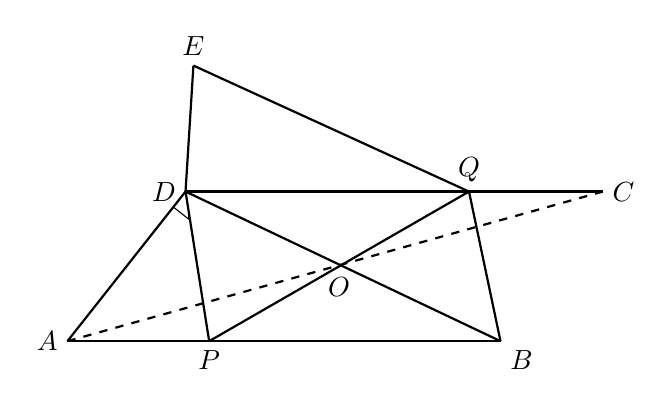
\begin{tikzpicture}[scale=1]
\coordinate (A) at (0,0);
\coordinate (P) at (1.8,0);
\coordinate (B) at (5.5,0);
\coordinate (D) at (1.5,1.9);
\coordinate (Q) at (5.1,1.9);
\coordinate (C) at (6.8,1.9);
\coordinate (E) at (1.6,3.5);
\coordinate (O) at (3.45,1.0);

\draw[thick] (A) -- (B);
\draw[thick] (A) -- (D) -- (B);
\draw[thick] (D) -- (C);
\draw[thick] (P) -- (Q) -- (B);
\draw[thick] (E) -- (D) -- (P);
\draw[thick] (E) -- (Q);
\draw[thick,dashed] (A) -- (C);

% right angle mark at D between AD and DP
\draw ($(D)!0.25cm!(A)$) -- ($($(D)!0.25cm!(A)$)!0.25cm!90:(A)$) -- ($(D)!0.25cm!(P)$);

\node[left] at (A) {$A$};
\node[below] at (P) {$P$};
\node[below right] at (B) {$B$};
\node[left] at (D) {$D$};
\node[above] at (Q) {$Q$};
\node[right] at (C) {$C$};
\node[above] at (E) {$E$};
\node[below=2pt] at (O) {$O$};
\end{tikzpicture}
\end{document}
